\clearpage 
\begin{figure}[t!]
  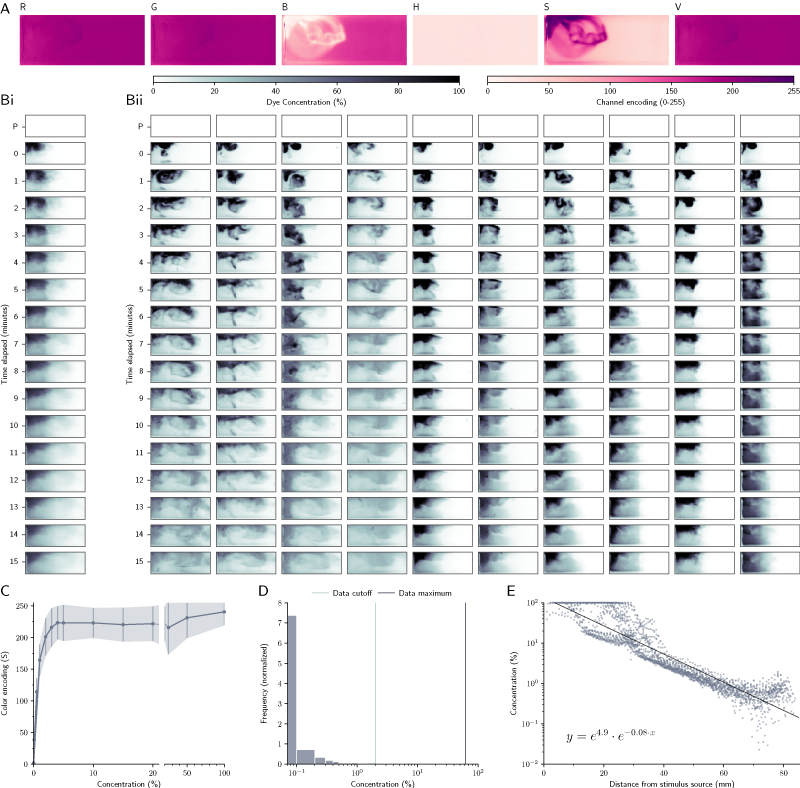
\includegraphics[width=\linewidth]{Figures/images/S2.eps}
  \caption{\textbf{Creating a concentration gradient map to analyze and model larval search behavior.} A: To quantify fluorescein dye diffusion, photographs were taken every minute using a Canon PowerShot ELPH 320 HS camera. Of the available color information channels (RGB, HSV), the saturation channel (S) contained the most information and was used to represent dye color throughout image analyses. Bi: Dye diffusion through time was quantified by the mean of all values in each 1mm2 area, linearly interpolated through time (n=10 experiments containing larvae). A control photograph was taken before the start of each experiment (P) but was not used to construct the chemical gradient map. Bii: Individual variation between trials. Each column represents data from one experiment through time. C: Dye color (S) was converted to raw concentration values using a standardization dataset of 13 reference concentrations. 20mL of each reference concentration was poured into the entire arena and photographed. D: Because 100${\mu}$L of dye is immediately diluted in the 20mL behavior arena water volume, reference concentration colors could not be used to directly convert color to ${\%}$ maximum concentration. Instead, the maximum concentration value was normalized to ${\geq}$95${\%}$ of all color measurements across all experiments. E: To create a concentration map for computational simulations in different arena sizes, we analyzed the relationship between concentration and distance from stimulus source at time=0. Concentration values for individual 1x1mm${^2}$ sections across all 10 experiments at time=0 (dots).
}
\end{figure}

\null
\vfill